\documentclass[12pt]{article}

% Language setting
% Replace `english' with e.g. `spanish' to change the document language
\usepackage[danish]{babel}

% Set page size and margins
% Replace `letterpaper' with `a4paper' for UK/EU standard size
\usepackage[a4paper,top=2cm,bottom=2cm,left=2cm,right=2cm,marginparwidth=1.75cm]{geometry}

% Useful packages
\usepackage{amsmath}
\newcommand{\Mod}[1]{\ (\mathrm{mod}\ #1)}

\usepackage[bottom]{footmisc}
\interfootnotelinepenalty=10000

\usepackage{graphicx}
\graphicspath{{img/}}


\usepackage[colorlinks=true, allcolors=black]{hyperref}
\usepackage[dvipsnames]{xcolor}
\usepackage{tikz}
\usetikzlibrary{calc}
\usepackage{anyfontsize}
\usepackage{tocloft}

\usepackage{hyperref}


\usepackage{wrapfig}


\usepackage{minted}
\usepackage[parfill]{parskip}

\title{Kryptografiske hashing algoritmer - MD5}
\author{Gustav Søndergaard Nybro}

\begin{document}


\begin{tikzpicture}[overlay,remember picture]
% Background color
\fill[
black!2]
(current page.south west) rectangle (current page.north east);

% Rectangles
\shade[
left color=Dandelion, 
right color=Dandelion!40,
transform canvas ={rotate around ={45:($(current page.north west)+(0,-6)$)}}] 
($(current page.north west)+(0,-6)$) rectangle ++(9,1.5);

\shade[
left color=lightgray,
right color=lightgray!50,
rounded corners=0.75cm,
transform canvas ={rotate around ={45:($(current page.north west)+(.5,-10)$)}}]
($(current page.north west)+(0.5,-10)$) rectangle ++(15,1.5);

\shade[
left color=lightgray,
rounded corners=0.3cm,
transform canvas ={rotate around ={45:($(current page.north west)+(.5,-10)$)}}] ($(current page.north west)+(1.5,-9.55)$) rectangle ++(7,.6);

\shade[
left color=orange!80,
right color=orange!60,
rounded corners=0.4cm,
transform canvas ={rotate around ={45:($(current page.north)+(-1.5,-3)$)}}]
($(current page.north)+(-1.5,-3)$) rectangle ++(9,0.8);

\shade[
left color=red!80,
right color=red!80,
rounded corners=0.9cm,
transform canvas ={rotate around ={45:($(current page.north)+(-3,-8)$)}}] ($(current page.north)+(-3,-8)$) rectangle ++(15,1.8);

\shade[
left color=orange,
right color=Dandelion,
rounded corners=0.9cm,
transform canvas ={rotate around ={45:($(current page.north west)+(4,-15.5)$)}}]
($(current page.north west)+(4,-15.5)$) rectangle ++(30,1.8);

\shade[
left color=RoyalBlue,
right color=Emerald,
rounded corners=0.75cm,
transform canvas ={rotate around ={45:($(current page.north west)+(13,-10)$)}}]
($(current page.north west)+(13,-10)$) rectangle ++(15,1.5);

\shade[
left color=lightgray,
rounded corners=0.3cm,
transform canvas ={rotate around ={45:($(current page.north west)+(18,-8)$)}}]
($(current page.north west)+(18,-8)$) rectangle ++(15,0.6);

\shade[
left color=lightgray,
rounded corners=0.4cm,
transform canvas ={rotate around ={45:($(current page.north west)+(19,-5.65)$)}}]
($(current page.north west)+(19,-5.65)$) rectangle ++(15,0.8);

\shade[
left color=OrangeRed,
right color=red!80,
rounded corners=0.6cm,
transform canvas ={rotate around ={45:($(current page.north west)+(20,-9)$)}}] 
($(current page.north west)+(20,-9)$) rectangle ++(14,1.2);

% Year
\draw[ultra thick,gray] ($(current page.center)+(5,2)$) -- ++(0,-3cm) node[midway, left=0.25cm, text width=5cm, align=right, black!75]{{\fontsize{25}{30} \selectfont \bf Studie Område \\[10pt] Projektet}} node[midway, right=0.25cm, text width=6cm, align=left, orange] {{\fontsize{72}{86.4} \selectfont 2022}};

% Title
\node[align=center] at ($(current page.center)+(0,-6.5)$) {
{\fontsize{26}{26} \selectfont {{Kryptografiske hashing algoritmer}}} \\[15pt] {\fontsize{28}{28} \selectfont {{MD5}}} \\[2cm]
{\fontsize{22}{22} \selectfont \textcolor{orange}{ \bf Gustav Søndergaard Nybro}}\\[10pt]
\Large  College360 - Teknisk Skole\\[3pt]
\Large  Programmering B \& Matematik A\\[3pt]
\Large  Gorm Drachmann \& Frans Carlsen\\[10pt]
\Large  8/12 - 2022};
\end{tikzpicture}
\thispagestyle{empty}
\newpage

\section*{Resumé}
 I dette projekt undforskes hashing algoritmer som en helhed, men mere specifikt også algoritmen MD5. MD5 er en gammel algoritme og betragtes usikker af mange. Den var dog stadig i brug, lang tid efter den blev erklæret usikker, at dens udvikler, Ron Rivest. 
Matematikken bag MD5 undersøges i detaljer, samt forudsætningerne for at kunne forstå MD5 algoritmen. Heriblandt en grundforståelse for boolsk algebra og diskret matematik. Derudover forklares hvert trin i processen til at genere et MD5 hash. Udover matematikken udforskes årsagen til, at MD5 ikke bruges længere, ved at lave en dybde gående analyse af sårbarhederne. Derudover demonstreres sårbarhederne blandt andet ved brug af en virkelighednær implementation. Denne implementation sammenlignes med en industristandard implementation af MD5 - selvom MD5 er betragtet som usikker. 


Udfra analysen og redegørelsen er det muligt at konkludere, at MD5, faktisk er en usikker algoritme, der ikke bør bruges i nogen sammenhæng. Den virkelighedsnære implementation med password i en database, viste hvor usikker MD5 er. Derudover viste kollisionsafsnittet, hvor simpelt det er at lave en MD5 kollision, som kan bruges til at udnytte systemer der bruger MD5 checksums som en sikkerhedsforanstaltning.   



\newpage



\renewcommand\cftsecfont{\large}
\renewcommand\cftsecpagefont{\large}
\renewcommand\cftsecafterpnum{\par\addvspace{7pt}}
\tableofcontents

\newpage
\section{Indledning}
I en tid hvor verdenen bliver mere og mere digitaliseret er det endnu vigtigere end før, at holde vores data sikker. Med adgang til en brugers konti'er er det muligt at overtage store dele af brugerens liv. En af de absolut vigtigste ting at holde hemmeligt for ondsindede tredjeparter er passwords. Dette er specielt vigtigt, hvis personen har tendens til at genbruge passwords som mange har. Med adgang til en brugers password, har man adgang til en meget stor del af deres liv. Skulle det ske, at en hacker opnåede adgang til en brugers password på en usikker tjeneste, er det sandsynligt, at det password også bliver brugt andre steder. 

Her kommer et af de absolut vigtigste værktøjer i spil - hashing algoritmer. De kan gøre det stortset umuligt for en hacker at opnå adgang til brugernes passwords. Men for at gøre dette kræver det en stærk og pålidelig hashing algoritme. Her kommer algorimen MD5 i spil, den betragtes af mange som en usikker hashing algoritme. Men hvis den er så usikker, hvorfor bliver den så stadig brugt? Derudover er det også interessant at udforske sårbarhederne, så man bedre kan beskytte sig mod dem. 

I denne rapport gennemgåes nogle brugssituationer for MD5 algoritmen, hvordan og hvornår den har været i brug. Derudover udforskes de forskellige sårbarheder med kode. Heriblandt bliver MD5 kollisioner udforsket og der gøres et forsøg på at opnå en MD5 kollision med to helt nye billeder. 




\section{Metoder}
Til programmeringdelen af SOP-opgaven udvikles der forskellige dele kode - en virkelighedsnær implementation og en hurtig demonstration af hvordan MD5 kan bruges. Derudover analyseres og sammenlignes kode, hvor der redegøres for sammenfald og eventuelle forskelle, i gennem hele rapporten. Til at fremstille koden bruges programmeringsproget Python (og i enkelte tilfælde nævnes C\#), da det er et simpelt og kraftigt sprog, hvor der hurtigt kan udvikles et godt produkt. Fordi Python er så udbredt, findes der også mange eksterne  biblioteker og klasser, der kan hjælpe med hurtigt at udvikle noget kode. Derudover er Python et let forståeligt sprog, da syntaksen minder meget om pseudo-kode. Det er derfor nemt at forestå, selv hvis man ikke har programmering erfaring med Python.     

Koden skrives i en IDE (Integrated Development Environment), hvilket er et program, hvor man kan skrive kode med en masse hjælpe værktøjer. I de fleste IDE'er oplyser den om fejl, hvis der skulle være nogle. De indeholde også ofte en "debug mode", der kan bruges til se præcis der sker i koden hele tiden, når det kører, for at fikse potentielle fejl. Til at udvikle Python kode kan der eksempelvis bruges PyCharm eller Visual Studio Code. Disse IDE'er indeholder også værktøjer som gør det nemt at forbinde til databaser og nemt finde dokumentation til forskellige metoder og klasser.  

For at udvikle koden kræver det kendskab til de forskellige biblioteker, der skal bruges. Her kan forskellige fora som StackOverflow bruges til at finde folk med lignende problemer og se deres løsninger. Derudover bruges den officielle dokumentation til bibliotekerne, til at undersøge de forskellige klasser og metoder, samt hvordan de bruges. 

Hvis der skulle opstå fejl i koden, bruges StackOverflow og dokumentationen, i samarbejde med "debug mode" til at fikse eventuelle problemer. 

For at holde styr på koden, bruges et VCS (Version Control System), der holder styr på ændringer i koden. Hvis man kommer til at lave noget forkert kode, er det derfor muligt at gå tilbage i historikken til noget, der virker. Det betyder også, at man nemt kan skrive kode på tværs af computere. Til denne opgave er der brugt Git som VCS og forbindes derved til GitHub, som er stedet Git forbinder og uploader koden til. GitHub bliver brugt af mange store virksomheder og projekter. 

For at kunne implementere og analysere MD5 algoritmen, udforskes matematikske emner udenfor pensum. Heriblandt udforskes boolsk algebra (logisk algebra), samt diskret matematik, hvor specifikt modulus begrebet bruges. Derudover udforskes forskellige matematiske notationer således, at matematikken kan opskrives på forskellige måder. 

\section{Intro om hashing algoritmer}
En hashing algoritme er blot en matematisk algoritme, der tager noget data som input og videregiver noget ulæselig- og utydelig data, som virker helt tilfældig. 
Det helt utydelige data kaldes for en "hash" (Se figur \ref{fig:hashing-algo-example}). 
Man kan ikke "gå baglens" med hashing algoritmer. 
Det er altså ikke muligt at producere rå tekst ud fra et hash. I teorien kan to forskellige input give samme hash - dette kaldes for en hash kollision. I sikre hashing algoritmer burde dette være matematisk usandsynligt, der findes dog nogle usikre algoritmer, hvor det er trivielt at opnå en kollision.


Der findes mange forskellige hashing algoritmer, men de har allesammen nogle ting til fælles \cite{Okta}:
\begin{enumerate}
\item De er allesammen baseret på matematik 
\item Længden af hashet, der bliver produceret, forbliver det samme - uanset længden af inputtet.
\item Algoritmen fungerer kun en vej 
\item De giver samme output med samme input - algoritmen skal være forudsigelig
\end{enumerate}


\begin{figure}[h]
\includegraphics[width=0.7\linewidth]{hashingWIKI.png} 
\centering
\caption{Hashing algoritmer \cite{wiki:hash}}
\label{fig:hashing-algo-example}
\end{figure}

Som det kan ses på \figurename{~\ref{fig:hashing-algo-example}}, betyder længden af inputtet ikke noget for længden af det endelige hash. Uanset hvilken hashing algoritme, der bliver brugt, forbliver længden altid det samme. Det er en sikkerhedsforanstaltning, der sikrer, at man ikke kan tyde på hashet, hvad inputtet kunne være. Derudover sikrer det også, at det er lige svært at 'gætte' hvad et hash kan repræsentere, selv hvis hashet kun var 1 byte (1 ASCII karakter). 


Hashing algoritmer bliver brugt i mange sammenhænge med datasikkerhed.
Man bruger faktisk hashing algoritmer hver dag uden at tænke over det.
Når man f.eks. skal logge ind på en hjemmeside, sender hjemmesiden en ens password i "hashet" format til databasen og tjekker, om de er ens.
Passwords bliver ikke opbevaret i normal tekst af flere grunde. 
En af de vigtigste grunde er for at sikre, at selv hvis en ondsindet person skulle få adgang til databasen, har de kun det hashede password og kan derfor ikke logge ind. 
\cite{Okta} 


Hashing bliver også brugt i andre sammenhænge. 
Når man downloader en fil fra internettet, kan man ikke være sikker på, at man har den rigtige fil, derfor er der ofte et hash på hjemmesiden. Med dette hash kan man så sammenligne hashet af den fil, man har downloadet, og det hash, der er opgivet på hjemmesiden. 
Hvis disse hashes er identiske, kan man være sikker på, at man har den rigtige fil, og ikke har modtaget en forkert fil. Dette kan bruges til to forskellige ting. Det kan bruges til at tjekke om filen er blevet 'ødelagt', mens den blev downloaded, da en enkelt lille fejl betyder, at hashet bliver noget helt andet. Derudover kan det sikre, at man ikke har fået en forkert fil, som en hacker eksempelvis har sendt med. \cite{techiedip_what_2012}




\section{MD5 hashing algoritme}

MD5 er en hashing algoritme udviklet i 1992 af Ron Rivest. MD5 blev udviklet som en mere sikker videreudvikling af den tidligere hashing algoritme MD4, men som det er tydeligt i dag, har den ikke bestået tidens prøve (dette uddybes lidt senere  i de kommende afsnit). De første MD algoritmer kom aldrig ud af laboratoriet, fordi de ikke var sikre nok. MD4 holdt også kun i et år, før der blev fundet en kollision. \cite{lake_md5_2021} 

MD5 algoritmen producerer altid et output der er 128 bit langt, hvilket kan (og ofte bliver) repræsenteres med hexadecimale tal \cite{rivest_md5_1992}. Hashet af teksten: \verb|MD5 SOP| kan eksempelvis repræsenteres med hexadecimaletal som \verb|f19c607bf61f5e03f115eefb9c3392da|. 

MD5 er en hashing algoritme og opfylder derfor alle krav, der er specificeret i afsnit 3. Dette kan også hurtigt testes med noget Python kode. Testen kan findes på \figurename{~\ref{code:md5-test}}.


\begin{figure}[!ht]
\begin{minted}[frame=lines,framesep=2mm,baselinestretch=1.2,linenos]{python}
import hashlib

print(hashlib.md5(b"MD5 SOP").hexdigest())
# Printer "f19c607bf61f5e03f115eefb9c3392da" i cmd

print(hashlib.md5(b"MD5 SOP").hexdigest())
# Printer "f19c607bf61f5e03f115eefb9c3392da" i cmd

print(hashlib.md5(b"Md5 SOP").hexdigest())
# Printer "7dab6061a04dd5327eddfed17f56a629" i cmd
\end{minted}
\caption{Simpel test af MD5 algoritmen i Python}
\label{code:md5-test}
\end{figure}
Koden i \figurename{~\ref{code:md5-test}} tester både om MD5 funktionen returnerer det samme hver gang, hvis inputtet er det samme, hvor stor forskel, store og små bogstaver kan have på det endelige resultat. MD5 algoritmen klarer begge tests. 

I linje 1 af koden importeres \verb|hashlib| biblioteket. Det indeholder en masse forskellige klasser og metoder der kan forskellige ting, som relaterer sig til hashing. Det indeholder eksempelvis \verb|md5| metoden, der bruges i det efterfølgende kode. 

I linje 3 printes MD5 hashet af strengen "MD5 SOP" hashet med MD5, til konsolen. Det fungerer ved at metoden \verb|md5|, fra klassen \verb|hashlib| kaldes. Denne metode tager en byte encoded streng af tekst og returnerer et objekt. En byte encoded streng er en datatype, hvor hver karakter i strengen repræsenteres med et tal fra 0-255 i stedet for et bogstav. En byte streng kan skrive således \verb|b'Streng'|, hvor \verb|b| indikerer, at det er en byte streng. 

Objektet der returneres indeholder en masse data, men for at få selve hashet ud, køres metoden \verb|.hexdigest()| på objektet. \verb|.hexdigest()| er en metode, der retunerer en streng af tekst, der indeholder en hexadecimal repræsentation af hashet. 


Det samme sker i linje 6 med samme tekst input for at demonstrere, at den samme tekst altid har samme hash. Den samme kode køres igen i linje 9, hvor det er en anden tekst end før (lille 'd' i 'MD5') for at demonstrere, at en lille ændring i inputtet kan ændre hele outputtet. Dette kaldes også for "The Avalanche effect" eller "Lavine effekten".

\begin{figure}[h]
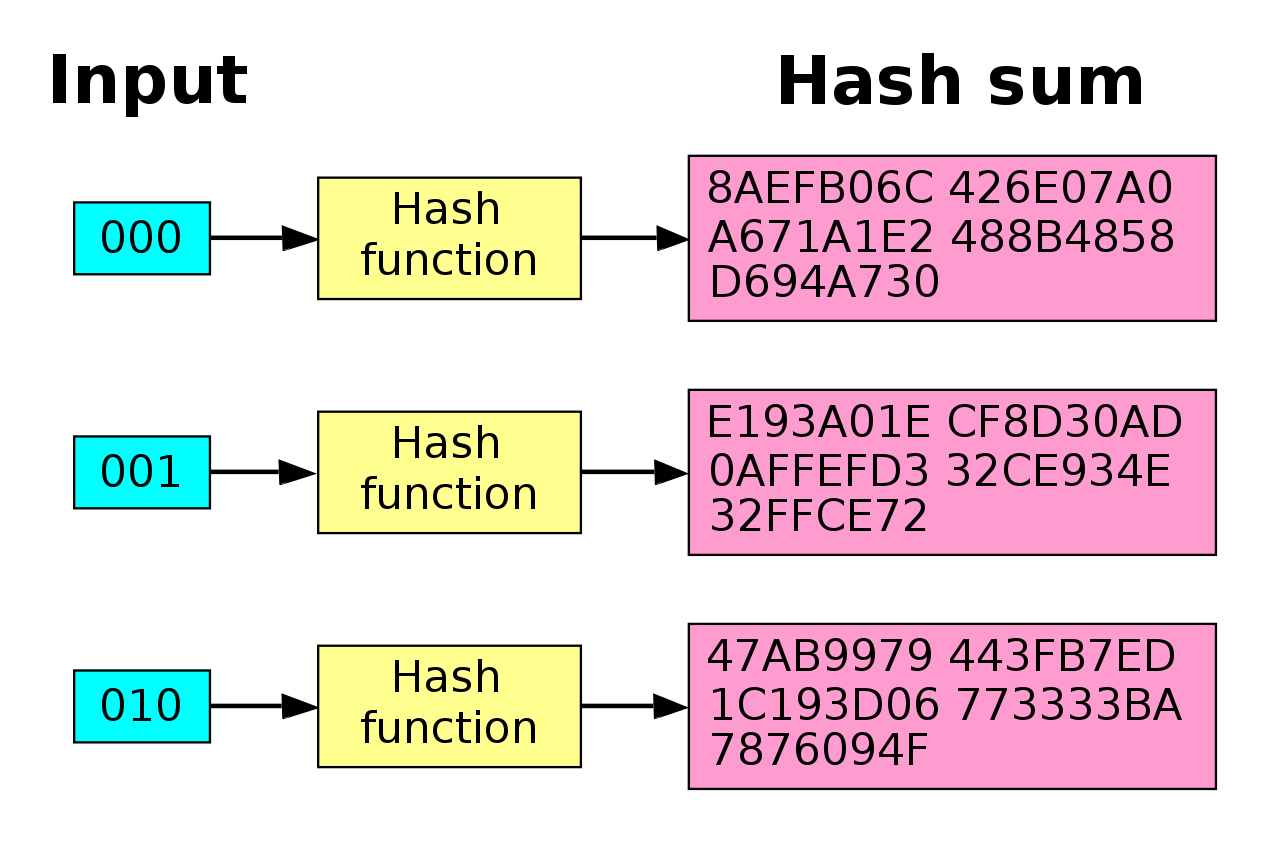
\includegraphics[width=0.7\linewidth]{Avalanche.png} 
\centering
\caption{Avalanche effekten illustreret \cite{wiki:avalance}}
\label{fig:avalanche-example}
\end{figure}

Dette fænomen er en meget vigtig sikkerhedsforanstaltning på alle hashing algoritmer. Lavine effekten siger, at outputtet skal have drastiske ændringer, selv ved minimale ændringer ved inputtet. Det betyder, at noget så simpelt som en ændring af et tegn burde ændre hele outputtet. Uden dette ville det teoretisk set være muligt at forudsige inputtet af et hash, såfremt man kender inputtet til et ligende hash. Derudover skal ændringen være uforudsigelig, så hashet ikke ændrer sig med et bestemt mønster ved samme type ændring. Et hash skal altså ikke ændre sig på en forudsigelig måde, hvis man eksempelvis sætter et punktum i slutningen af en sætning i forhold til uden punktum. En hashing funktion bør opføre sig som illustreret på \figurename{~\ref{fig:avalanche-example}}, hvor der er drastiske ændringer i output ved en minimal ændring i inputtet \cite{al-kuwari_cryptographic_nodate}.



\section{MD5 matematik og virkemåde}
\subsection{Definitioner}
Før MD5 algoritmen analyseres, er det vigtigt at definere nogle begreber. Et \verb|ord| er beskrevet som en størrelse på 32 bit, og en \verb|byte| er beskrevet som en størrelse på 8 bit. En \verb|block| er beskrevet som en størrelse på 512 bit. En bit er den mindste størrelse, der bliver brugt indenfor computer området. Den kan enten være 1 eller 0, og kan sættes sammen således, at det former et binært tal. Disse binære tal kan repræsentere alle værdier af tal og tegn. 

\subsection{Modulus}
Det er vigtigt at have en grundforståelse for modulus, for at kunne implementere MD5 algoritmen. Modulus kan også forståes som resten efter heltalsdivision. 
Modulus har følgende notation, som kan ses i \equationautorefname{~\ref{math:modulo-eq}}:
\begin{equation}
a\equiv b \Mod{n}
\label{math:modulo-eq}
\end{equation}
\equationautorefname{~\ref{math:modulo-eq}} kan forståes som a modulus n er lig b. Man kan tage følgende eksempel i \equationautorefname{~\ref{math:modulo-example-1}}
\begin{equation}
7\equiv 1 \Mod{3}
\label{math:modulo-example-1}
\end{equation}
Hvis man med heltalsdivision dividerer 7 med 3, resulterer det i 2 med 1 til rest. 
\begin{equation}
7=3\cdot 2 + 1
\label{math:modulo-example-1-calc}
\end{equation}
De fleste programmering sprog, bruger derfor en anden notation, som kan ses i \equationautorefname{~\ref{math:modulo-example-2}}
\begin{equation}
7 \ \% \ 3
\label{math:modulo-example-2}
\end{equation}

Modulus bliver brugt til mange hashing algoritmer, da det er umuligt at "gå baglens" med modulus, eftersom der er mange forskellige ligninger, der kan give samme resultat. \(7\equiv 1 \Mod{3}\) og \(9\equiv 1 \Mod{4}\) er begge sande udtryk, der har samme resultat. Det er derfor umuligt at vide hvilke tal, det startede med, hvis man kun kender resultatet. Det er dog dog nemt at tjekke resultatet, hvis man har begge tal det startede med. 


\subsection{Boolsk Algebra}
Ud over at kunne forstå modulus er det også vigtigt at have en grundforståelse for boolsk algebra. Det vigtigste er at kunne forstå de logiske operatorerne, der bliver brugt - eksempelvis AND eller OR. For at kunne implementere MD5 algoritmen udføres alle disse operatorer "bitwise", hvilket betyder, at man sammenligner og omregner alle tal og tegn til binære tal og tilfører operationen en bit afgangen.  



\subsubsection{AND}
Ved \verb|AND| er outputtet sandt (betegnes med 1), hvis begge input er sande, ellers er det falsk. Med matematisk notation betegnes \verb|AND| som \(\wedge\), og med programmeringsnotation, betegnes \verb|AND| ofte\footnotemark[1] med \(\&\). Dog bruges \verb|AND| i mange tilfælde for simplicitet. 
\begin{equation}
\begin{split}
\mathsf{     1001 \ (decimal\ 9) } \\
\mathsf{AND\ 0011 \ (decimal\ 3) } \\
\mathsf{   = 0001 \ (decimal\ 1) }
\end{split}
\end{equation}

\subsubsection{OR}
Ved \verb|OR| er outputtet sandt, hvis et eller begge input er sande, ellers er det falsk. Med matematisk notation, betegnes \verb|OR| som \(\vee\), og med programmeringsnotation betegnes \verb|OR| ofte\footnotemark[1] med \(|\). Igen bruges \verb|OR| ofte isstedet for matematisk notation for simplicitet.  

\begin{equation}
\begin{split}
\mathsf{     1001}& \ \mathsf{(decimal\ 9 ) } \\
\mathsf{OR \ 0011}& \ \mathsf{(decimal\ 3 ) } \\
\mathsf{   = 1011}& \ \mathsf{(decimal\ 11) }
\end{split}
\end{equation}

\subsubsection{XOR}
Ved \verb|XOR| er outputtet sandt, hvis kun et input er sandt, ellers er det falsk. Med matematisk notation betegnes \verb|XOR| som \(\oplus\), og med programmeringsnotation betegnes \verb|XOR| ofte\footnotemark[1] med \textasciicircum. Igen bruges \verb|XOR| ofte isstedet for matematisk notation for simplicitet.  
\begin{equation}
\begin{split}
\mathsf{     1001}& \ \mathsf{(decimal\ 9 ) } \\
\mathsf{XOR\ 0011}& \ \mathsf{(decimal\ 3 ) } \\
\mathsf{   = 1010}& \ \mathsf{(decimal\ 10) }
\end{split}
\end{equation}

\footnotetext[1]{Når der skrives om de fleste tilfælde i programmering notation menes der, at de fleste og mest brugte programmeringsprog bruger den beskrevne notation. I hele denne rapport bruges den beskrevne notation (medmindre andet er specificeret). Der findes andre notationer i andre sprog, dog bruges disse sprog ikke i denne beskrivelse af MD5.}

\subsubsection{NOT}
Den sidste vigtige logiske operator er \verb|NOT|. \verb|NOT| inverterer blot inputtet, således at outputtet er den modsatte binære repræsentation af inputtet. Derfor kan \verb|NOT| kun bruges på et input adgangen. Med matematisk notation betegnes \verb|NOT| med \(\neg\), og betegnes med $\sim$ i de fleste tilfælde med programmeringnotation\footnotemark[1].

\begin{equation}
\begin{split}
\mathsf{NOT\ 0011}& \mathsf{\ (decimal\ 3 ) } \\
\mathsf{   = 1100}& \mathsf{\ (decimal\ 12) }
\end{split}
\end{equation}



\subsection{Bit rotationer}
\begin{wrapfigure}{r}{0.3\textwidth}
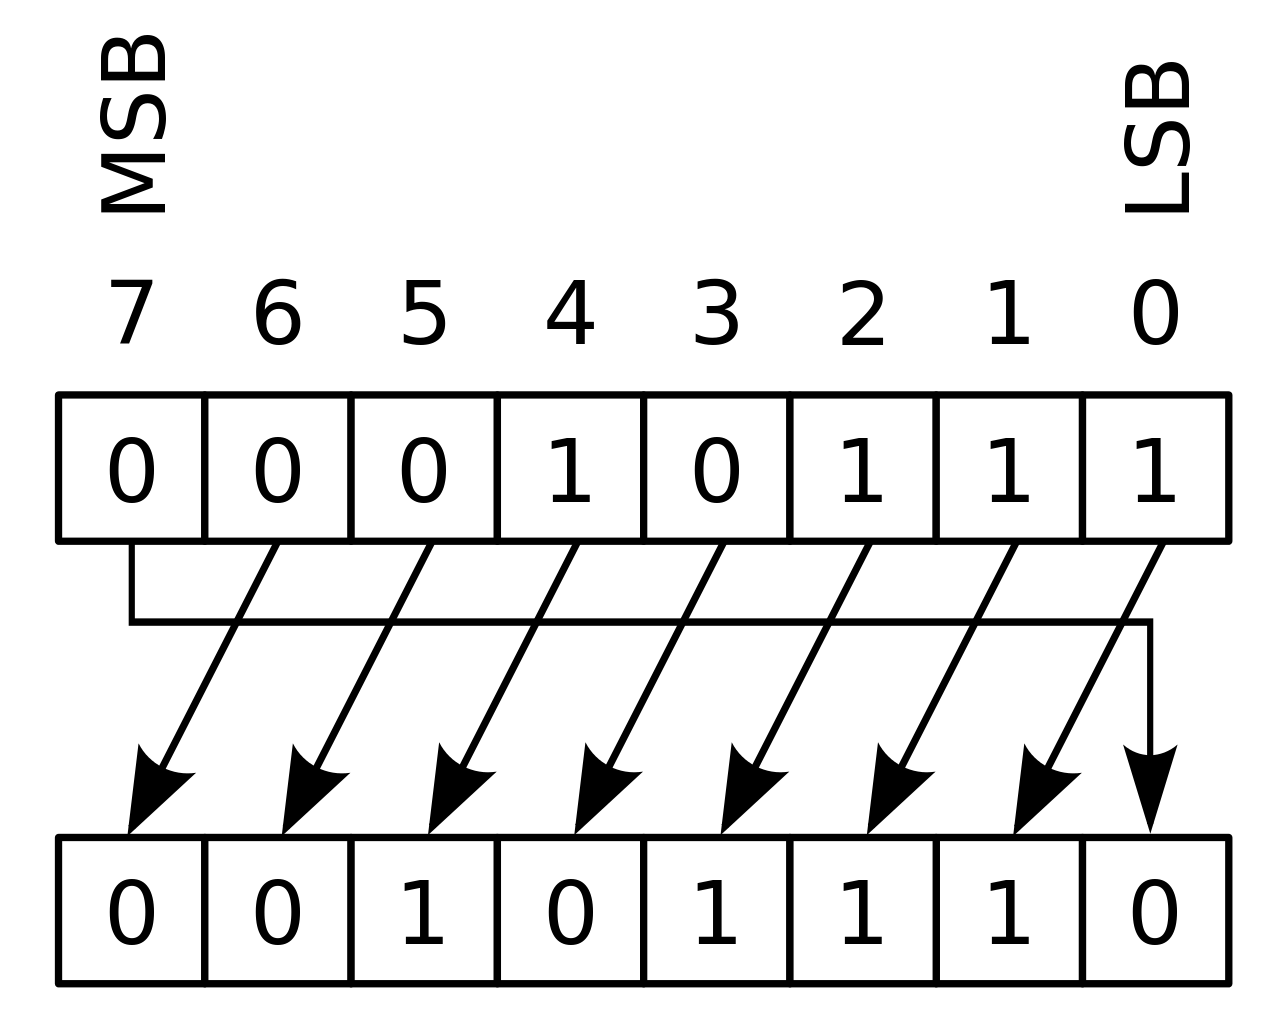
\includegraphics[width=0.8\linewidth]{Rotate_left.png} 
\caption{En enkelt rotation til venstre illustreret \cite{wiki:circular}}
\label{fig:left-rotate-example}
\end{wrapfigure}

En bit rotation er også et vigtigt værktøj når MD5 skal implementeres. En bitrotation udføres med binære tal. En bit rotation kan ske til højre eller venstre. Hvis man eksempelvis roterer til venstre med 3, rykkes de tre mest signifikante bits\footnotemark[2] til højre side af tallet og bliver derfor de tre mindst signifikante bits. På \figurename{~\ref{fig:left-rotate-example}}, illustreres en rotation med 1, til venstre. Denne process gentages i alt tre gange, hvorefter sekvensen er blevet roteret med 3 til venstre. 


En bit rotation består et \verb|bitshift|, som er en proces, hvor man blot skubber bits med en bestemt længde (uden nødvendigvis at ændre MSB til LSB, men blot tilføjer mere data). I programmering repræsenteres et bitshift ofte \footnotemark[1] som \( a << n \), hvor \verb|a| er bits, der skal forskydes og, \verb|n| er mængden, de skal forskydes med.  Derudover skal de forskudte bits sættes til den modsatte side - forskyder man eksempelvis til venstre, gøres MSB til LSB. 


\footnotetext[2]{De bits der ændrer størrelsen af tallet mest, dvs. der er mest til venstre i et binært tal. Binære tal er skrevet i "big endian", hvilket betyder at tal længst mod venstre har størst betydning for hele tallets størrelse. Decimaltal fungerer også efter dette princip. De mest signifikante bits kendes også ofte som MSB for "most signifikante bits". Det modsatte er mindst siginifaknte bits (LSB, "least siginificant bits"), der står længst til højre. }


\subsection{MD5 algoritmen}
Følgende redegørelse for MD5 algoritmen er en mere uddybet version af det officielle dokument, der specificerer MD5 standarden. Dette dokument blev skrevet af Ron Rivest i 1992 \cite{rivest_md5_1992}.

\footnotetext[3]{ACSII står for "American Standard Code for Information Interchange", hvilket betyder, at det er en standard, der beskriver hvordan bogstaver og tegn, kan repræsenteres med binær form}

\subsubsection{Trin 1 - Input besked}
Første trin i at implementere og beregne et MD5 hash, er at omdanne input beskeden til binær repræsentation, så algoritmen kan behandle data'en korrekt. Dette gøres ved brug af en ASCII tabel \footnotemark[3], hvor  hvert bogstav omdannes til en værdi, repræsenteret i binær.

Det kunne eksempelvis se sådan ud: 

\begin{equation}
\begin{split}
&\mathsf{01000111 \ 01110101 \ 01110011 \ 01110100} \\
&\mathsf{01100001 \ 01110110 \ 01110011 \ 00100000} \\
&\mathsf{01001101 \ 01000100 \ 00110101 \ 00100000} \\
&\mathsf{01010011 \ 01001111 \ 01010000 } 
\end{split}
\label{step-1-binary}
\end{equation}
\equationautorefname{~\ref{step-1-binary}} er en binær repræsentation af teksten "Gustavs MD5 SOP" oversat ved brug af en ASCII tabel. For at undgå at hashet ændrer længde afhæning af længden af inputtet påføres "padding" som starter med 1 efterfulgt 0'er indtil længden af inputtet er 448 bit, hvilket er længden af en block minus 8 byte. Disse 8 bytes skal bruges til at definere længden af input beskeden. Mængden af 0'er, der skal påføres efter beskeden, kan beregnes: \(448-1-n\), hvor \verb|n| beskriver længden af input beskeden og -1 er fratrækkelsen af det første 1, der sættes efter beskeden. 


Et færdig resultat, efter padding, kunne se ud som \equationautorefname{~\ref{step-2-binary}}:

\begin{equation}
\begin{split}
&\mathsf{01000111 \ 01110101 \ 01110011 \ 01110100 \ = 47757374 }\\
&\mathsf{01100001 \ 01110110 \ 01110011 \ 00100000 \ = 61767320 }\\
&\mathsf{01001101 \ 01000100 \ 00110101 \ 00100000 \ = 4d443520 }\\
&\mathsf{01010011 \ 01001111 \ 01010000 \ 10000000 \ = 534f5080 }\\
&\mathsf{00000000 \ 00000000 \ 00000000 \ 00000000 \ = 00000000 }\\
&\mathsf{00000000 \ 00000000 \ 00000000 \ 00000000 \ = 00000000 }\\
&\mathsf{00000000 \ 00000000 \ 00000000 \ 00000000 \ = 00000000 }\\
&\mathsf{00000000 \ 00000000 \ 00000000 \ 00000000 \ = 00000000 }\\
&\mathsf{00000000 \ 00000000 \ 00000000 \ 00000000 \ = 00000000 }\\
&\mathsf{00000000 \ 00000000 \ 00000000 \ 00000000 \ = 00000000 }\\
&\mathsf{00000000 \ 00000000 \ 00000000 \ 00000000 \ = 00000000 }\\
&\mathsf{00000000 \ 00000000 \ 00000000 \ 00000000 \ = 00000000 }\\
&\mathsf{00000000 \ 00000000 \ 00000000 \ 00000000 \ = 00000000 }\\
&\mathsf{00000000 \ 00000000 \ 00000000 \ 00000000 \ = 00000000 }\\
&\mathsf{00000000 \ 00000000 \ 00000000 \ 00000000 \ = 00000000 }\\
&\mathsf{00000000 \ 00000000 \ 00000000 \ 01111000 \ = 00000078 }
\end{split}
\label{step-2-binary}
\end{equation}

\equationautorefname{~\ref{step-2-binary}} er en binær repræsentation af teksten "Gustavs MD5 SOP" med padding påsat, samt længden af den originale tekst. Derudover er teksten på højre side af lighedstegnet, det forrige ord (32 bit) repræsenteret med hexadecimale tal (base 16). Blokken inddeles 16 ord (af 32 bit hver). Hvert ord kaldes for $M_i$, hvor $i$ beskriver indeksværdien - altså hvilket ord det er på listen. $M_0$ vil derfor blive $47757374$ og $M_{15}$ bliver $00000078$. \footnotemark[4]

\footnotetext[4]{Da dette er en programmerings algoritme, er den også designet med programmering i mende, hvilket er derfor listen starter ved 0 istedet for 1. I de fleste programmeringsprog starter lister (arrays) ved 0. Derudover starter løkker (et koncept der udfører en handling gentagende gange) også med 0. }

\subsubsection{Trin 2 - initialiser vektorerne}
Til at starte operationen initialiseres 4 variable, der til start indeholder standard værdier, men gennem forskellige operationer ændrer værdi. Disse variable har følgende startværdier:

\begin{equation}
\begin{split}
&\mathsf{A: 01\ 23\ 45\ 67}\\
&\mathsf{B: 89\ ab\ cd\ ef}\\
&\mathsf{C: fe\ dc\ ba\ 98}\\
&\mathsf{D: 76\ 54\ 32\ 10}
\end{split}
\label{step-2-word-buffers}
\end{equation}

Værdierne i \equationautorefname{~\ref{step-2-word-buffers}} er repræsenteret i hexadecimale tal. Disse specifikke tal kaldes også for initialiseringsvektorer og skal bruges flere steder i operationen. 

\subsubsection{Trin 3 - definer hjælpefunktioner}
For at kunne generere et hash, er der brug for matematiske funktioner. Disse matematiske funktioner består af forskellige operationer fra boolsk algebra og hedder (F, G, H, I). 
Funktionerne kan nemmest udtrykkes med matematisk notation, som er vist i \equationautorefname{~\ref{step-3-aux-func}}

\begin{equation}\label{step-3-aux-func}
\begin{split}
\mathsf{F(B, C, D)} & = \mathsf{(B\wedge C)\vee(\neg B\wedge D)}    \\
\mathsf{G(B, C, D)} & = \mathsf{(B\wedge D)\vee(C\wedge \neg D)}    \\
\mathsf{H(B, C, D)} & = \mathsf{B \oplus C \oplus D}                \\
\mathsf{I(B, C, D)} & = \mathsf{C \oplus (B \vee \neg D)}
\end{split}
\end{equation}

\subsubsection{Trin 4 - Processen}
\begin{figure}[h]
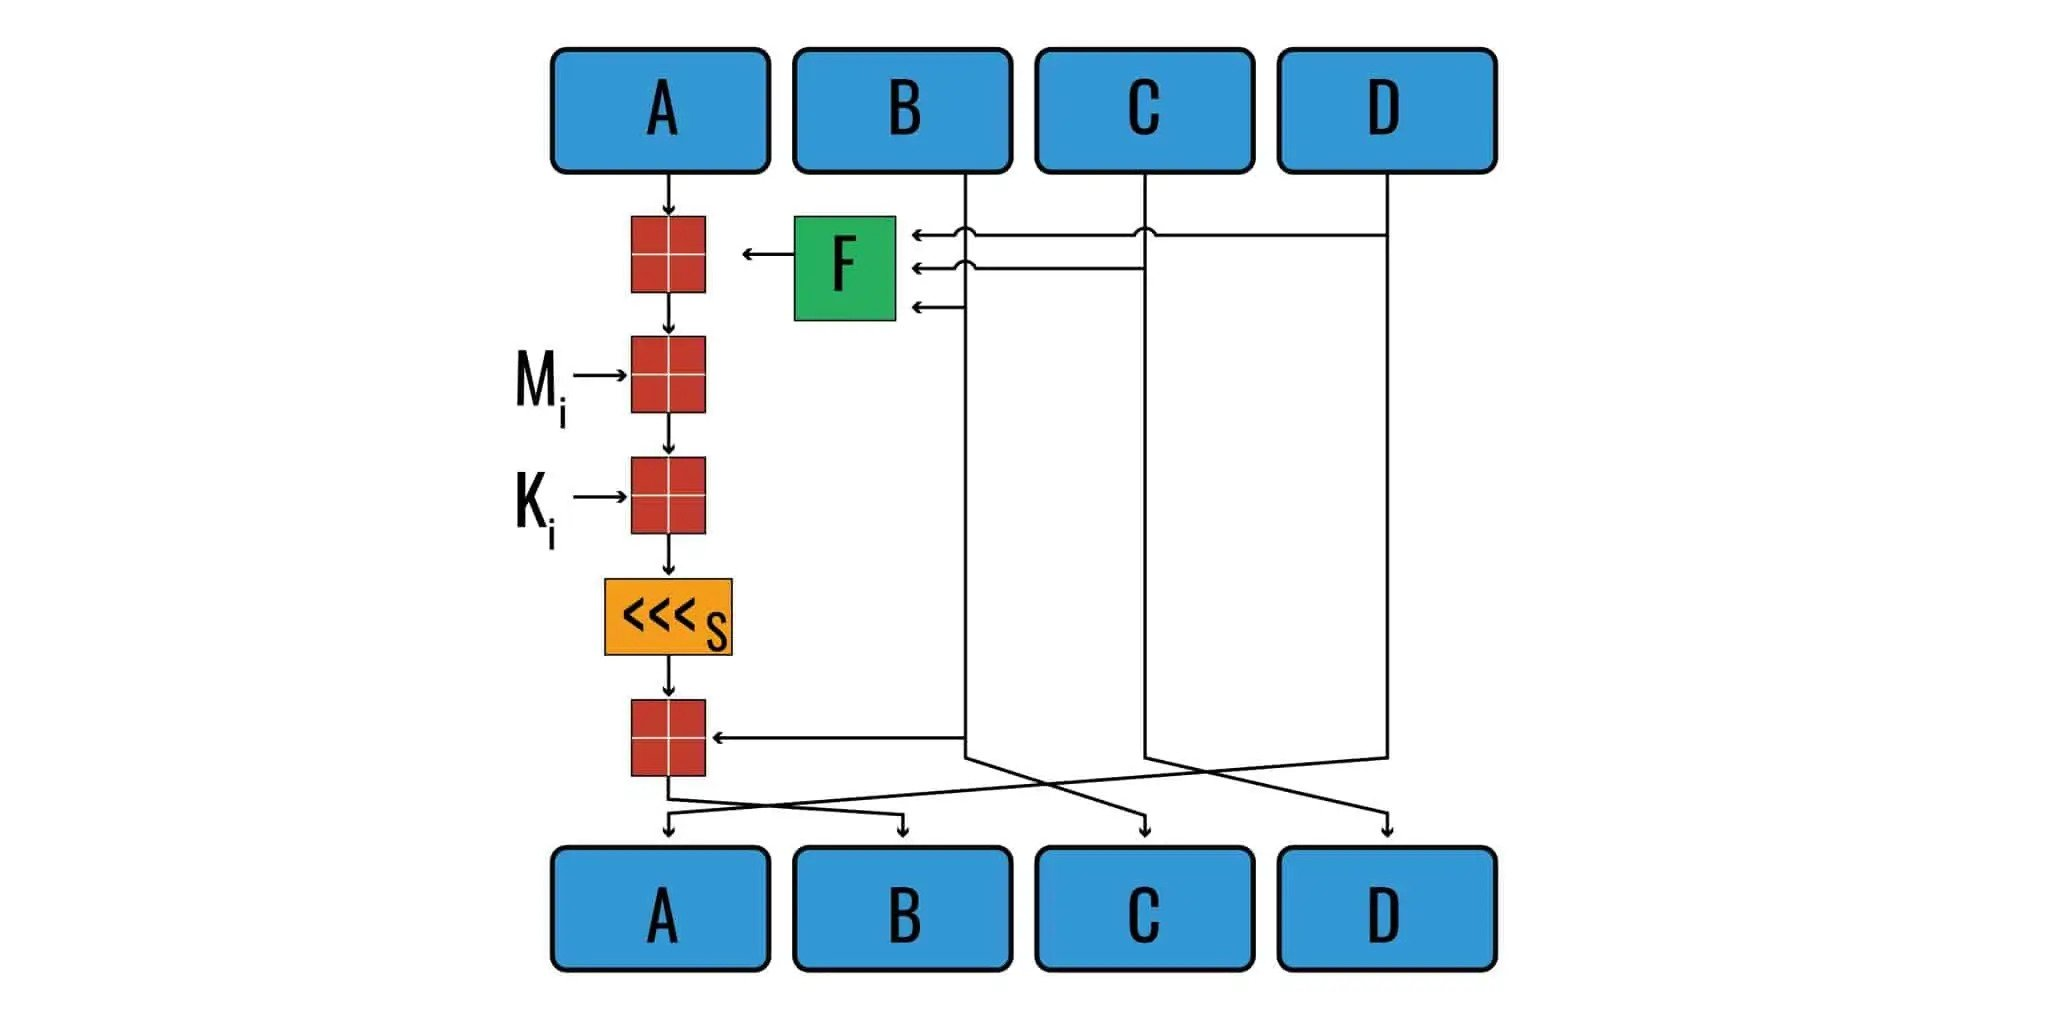
\includegraphics[width=1\linewidth]{hashing-round.jpg} 
\centering
\caption{Brugen af hjælpefunktioner illustreret \cite{lake_md5_2021}}
\label{fig:aux-func-used}
\end{figure}

\figureautorefname{~\ref{fig:aux-func-used}} illustrerer, hvordan hjælpefunktionerne bliver brugt til at generere et MD5 hash. Hver af de røde kasser illustreret, er et symbol for \verb|modulær additions| funktion. Funktionen tager to input og returnerer et. Funktionen kan beskrives med \equationautorefname{~\ref{step-4-func}}:

\begin{equation}\label{step-4-func}
(x+y) \equiv o \Mod{2^{32}}
\end{equation}

I \equationautorefname{~\ref{step-4-func}} er $x$ og $y$ de to input, som funktionen tager, og $o$ er outputtet af funktionen modulo $2^{32}$ operatiionen udføres på summen af $x+y$ for at undgå, at resultatet bliver for stort. 

Det er også muligt at skrive \equationautorefname{~\ref{step-4-func}} med programmeringsnotation, som vist på \figureautorefname{~\ref{code:step-4-mod_add}}

\begin{figure}[!ht]
\begin{minted}[frame=lines,framesep=2mm,baselinestretch=1.2,linenos]{python}
o = (x+y) % 2**32
\end{minted}
\caption{\equationautorefname{~\ref{step-4-func}} i programmerings notation}
\label{code:step-4-mod_add}
\end{figure}


I sprog uden $**$ operatoren (som betegner en eksponent), findes der metoder til at beregne tallet. Betragt eksempelvis \figureautorefname{~\ref{code:step-4-mod_add-c}}, som er et eksempel i sproget \verb|C#|


\begin{figure}[!ht]
\begin{minted}[frame=lines,framesep=2mm,baselinestretch=1.2,linenos]{csharp}
using System;

namespace PowTest{
    class Program{
        static void Main(string[] args){
            double a = Math.Pow(2, 32); // a = 4294967296
            Console.WriteLine(a); // Skrive "4294967296" til cmd
        }
    }
}
\end{minted}
\caption{\equationautorefname{~\ref{step-4-func}} i programmeringsnotation}
\label{code:step-4-mod_add-c}
\end{figure}
I \figureautorefname{~\ref{code:step-4-mod_add-c}} initialiseres en variabel \verb|a| med type \verb|double|, hvilket betyder, at den kan indeholde decimaltal samt store tal. \verb|a| sættes lig med resultatet af metoden \verb|Pow()| fra klassen \verb|Math|, som bliver importeret i linje 1. Udover den beskrevne kode er det blot \verb|C#| standard kode, der er nødvendigt for at kunne kompilere og køre koden. 

Det første trin i processen illustreret på \figureautorefname{~\ref{fig:aux-func-used}} er en modulær addition med resultatet af funktionen F (som beskrevet i Trin 3) og variablen A. Eftersom det er første gang processen køres har A samme værdi som initaliseringvektoreren A. De efterfølgende gange, er A blot værdien af variablen A. 

I det efterfølgende trin udføres modulær addition igen, med resultatet fra den tidligere funktion, samt beskeden med indeks $i$ ($i$ beskriver hvor mange gange løkken er blevet gentaget og starter ved 0) fra Trin 1. Eftersom det er første gang, processen bliver udført, er $i=0$ og næste gang vil i være $i=1$. 

I næste trin udføres igen modulær addition med resultatet fra den tidligere funktion, samt værdien fra funktionen K. Funktionen K kan beskrives med \equationautorefname{~\ref{step-4-sin-func}}.

\begin{equation}\label{step-4-sin-func}
K = | \sin{i+1} | \cdot 2^{32}
\end{equation}

I \equationautorefname{~\ref{step-4-sin-func}} tages den absolutte værdi af $\sin{i+1}$, hvor $i$ er den samme indeksværdi, der bruges i foregående funktion. Derudover ganges værdien med $2^{32}$. Dette er en konstant, der bruges i alle implementationer af MD5, og det er derfor også muligt at udregne dem på forhånd og blot bruge dem som tabelværdier.  

I næste trin sker der en bitrotation, hvor resultatet fra den forhåndværende funktion forskydes med en standardværdi. Disse standardværdier følger et bestemt mønster. Mønsteret har værdierne $\mathsf{7; 12; 17; 22}$, der gentages. Det betyder, at bruges værdien 7 eksempelvis, både i første og femte iteration af løkken. 

I den sidste funktion udføres en modulær addition (som beskrevet med \equationautorefname{~\ref{step-4-func}}), med resultatet fra den tidligere funktion, samt værdien i variablen B. Eftersom dette er første gang processen kører er variablen B lig værdien af initaliseringsvektoreren B. 

Til sidst i processen forskydes værdierne en gang til højre, hvilket betyder at værdien af A indsættes i B, B indsættes i C, C indsættes i D og D indsættes i A, næste gang processen udføres. 

Denne processen gentages 16 gange i streg, hvorefter trin 5 i gangsættes. 

\subsubsection{Trin 5 - G}
De kommende tre trin minder meget om de første trin og der er kun få forskelle. De kommende 3 trin, gentager Trin 1 - 4, blot med få ændringer af værdierne der bruges.

På dette trin bruges der hjælpegunktionen G, i stedet for F (begge er beskrevet i trin 3). Derudover indekses listen med beskeden med en anden formel, for at skifte rækkefølgen af beskeden. Denne formel kan beskrives som \equationautorefname{~\ref{step-5}}, hvor $i$ er det antal gange som løkken er udført, og $o$ er det tal, der skal bruges for at indeksere listen af beskeden. 
\begin{equation}\label{step-5}
(5\cdot i + 1) \equiv o \Mod{16}
\end{equation}

Derudover skal den modificerede formel for konstanten $K_i$ bruges, som vises i \equationautorefname{~\ref{step-5-2}} \footnotemark[5].
\begin{equation}\label{step-5-2}
K=| \sin{i+1+16} | \cdot 2^{32}
\end{equation}

Til sidst udføres bitrotation med et andet mønster, hvilket har talrækken $\mathsf{5;9;14;20}$. Udover disse trin er processen den samme. 

\subsubsection{Trin 6 - H}
Efter 16 runder i processen fra trin 5, skal der nu udføres 16 runder med H funktionen i stedet for G eller F funktionen. 
Derudover skal der igen bruges en anden formel til at indekse listen med besked ord. Den formel er beskrevet i \equationautorefname{~\ref{step-6}}
\begin{equation}\label{step-6}
(3\cdot i + 5) \equiv o \Mod{16}
\end{equation}

Der skal igen også bruges en modificeret formel til at beregne konstanten $K_i$, som ses i  \equationautorefname{~\ref{step-6-2}}\footnotemark[5].
\begin{equation}\label{step-6-2}
K=| \sin{i+1+32} | \cdot 2^{32}
\end{equation}


Igen udføres bitrotation med en anden talrække. Denne talrække er $\mathsf{4;11;16;23}$

\subsubsection{Trin 7 - I}
I trin7 bruges hjælpefunktionen I. 

Den sidste formel til at indekse besked listen er som beskrevet i \equationautorefname{~\ref{step-7}}
\begin{equation}\label{step-7}
(7\cdot i) \equiv o \Mod{16}
\end{equation}

Igen bruges der en anden formel til at beregne konstanten $K_i$, som ses i \footnotemark[5]. \equationautorefname{~\ref{step-7-2}}.
\begin{equation}\label{step-7-2}
| \sin{i+1+48} | \cdot 2^{32}
\end{equation}

Den afsluttende talrække til udførsel af bitrotation er: $\mathsf{6;10;15;21}$

\footnotetext[5]{Formlen er faktisk ikke anderledes for hver trin, men fordi formlen er lavet til at beregnes værdier fra 0 - 64 og ikke 0 - 16, lægges der en ekstra værdi til. Da et trin kun gentages 16 gange og der er fire trin (16 * 4 = 64), og der ikke kun er en trin med 64 runder, pålægges den ekstra værdi. }
\subsubsection{Trin 8 - Afslutning}
Efter alle fire hjælpefunktioner og tilhørende trin er blevet udført, skal der blot ske to handlinger, inden der er fremstillet et hash. 

Første trin er at udøre modulær addition (ligesom de tidligere trin), men i stedet bruges resultatet af trinene og den oprindelige initaliseringsvektor til at fremstille en del af hashet. Det betyder at variablen A adderes sammen med initaliseringsvektoreren A. Dette fremstiller en del af hashet.

Det sidste trin dikterer at man sætter de fire del-hashes sammen, hvilket resulterer i et helt MD5 hash. 

\section{Usikkerheder og implementation}
\subsection{Hurtig MD5 generering}
En af de store sårbarheder i MD5 algoritmen er, hvor hurtigt man kan generere hashes og hvor "lille" mængden af hashes, der kan eksistere med algoritmen \cite{ntantogian_evaluation_2019}. Det er muligt at generere cirka 21 milliarder hashes i sekundet med et gennemsnitligt 6 år gammelt grafikkort \cite{ntantogian_evaluation_2019}. Det betyder derfor, at man hurtigt kan generere en stor mængde hashes på meget kort tid. Hvis man får adgang til en database, er det muligt at generere hashes for mange passwords, når man kender saltet. Et salt er en streng af tekst der sættes før- eller efter et password, som dernæst hashes. Et salt er tilfældigt genereret, når brugeren opretter sig. Dette sikrer, at der ikke er to ens hashes i en database. Det gør det også sværere for en hacker, der har opnået adgang til databasen, da de individuelt skal 'gætte' passwordet og saltet for hver bruger. Hvis der ikke gøres brug af salt, kræver det kun at man gætter et password en gang. 

\subsubsection{Kode}
For at demonstrere en sårbarheden hvor man kan generere en stor mængde hashes hurtigt, er der blevet udviklet en virkelighedsnær implementation af MD5 hashing. Derudover er der blevet udviklet en implementation uden salt og en med salt. 

Koden er udviklet i Python for at gøre udviklings processen kortere, da der er mange biblioteker indbygget. Derudover er koden udviklet, for at fremvise en mulig implementation af MD5, hvilket betyder at der er nogle få sårbarheder i koden. 

I koden er der brugt en SQLite3 database, som er en database, der kan gemmes i en enkelt fil. Dette gør det nemmere at køre koden på flere forskellige computere, da der blot skal overføres en fil. Der tages udgangspunkt i to funktioner, som kan oprette en bruger. Det resterende kode kan findes i bilag, her findes blandt andet koden, der opretter forbindelse til databasen og koden, der logger brugeren ind. 

\subsubsection{Kode der opretter en bruger}

\begin{figure}[ht]
\begin{minted}[frame=lines,framesep=2mm,baselinestretch=1.2,linenos,breaklines]{python}
def create_user(username, password):
    # Hasher passwordet
    hashed_password = hashlib.md5(password.encode()).hexdigest()

    # Laver en SQL kommando der henter alle brugernavnet brugeren har indsat
    c.execute("SELECT * FROM credentials WHERE username = ?", (username,))
    # Hvis der ikke er nogen brugere med det brugernavn
    if c.fetchone() is None:  
        # Laver en SQL kommando der indsætter brugernavn og password i db
        c.execute("INSERT INTO credentials(username,password) VALUES (?,?)", (username, hashed_password))
        conn.commit()
        print(f"User {username} created")

    else:  
        # Printer at der allerede er en bruger med det brugernavn
        print("User already exists")
\end{minted}
\caption{Funktion der kan oprette en bruer uden salt}
\label{code:create-user-wo-salt}
\end{figure}


På \figureautorefname{~\ref{code:create-user-wo-salt}} vises et udsnit af koden, der indeholder en funktion, som kan oprette en bruger (uden salt) i databasen, samt tjekke om der allerede findes en bruger med brugernavnet. I linje 1 defineres funktionen. Den tager et brugernavn og password som input. Brugernavn og password indsættes, når funktionen kaldes senere i koden. I linje 3, hashes passwordet, som brugeren har indsat. Det sker ved brug af funktionen \verb|md5|, som også blev brugt i \figurename{~\ref{code:md5-test}}. Denne gang bruges \verb|.encode()| i stedet for \verb|b''|. Det er samme princip, blot to forskellige måder at skrive det på. De laver begge to tekst strengen om til en række bytes. 

Variablerne \verb|c| og \verb|conn| er variabler, der er blevet oprettet tidligere i koden. De er beskrevet i detaljer i selve koden. De to variabler indeholder, objektene som bruges til at læse og skrive til databasen. 

I linje 6 bliver der eksekvereret en linje SQL i databasen. Denne linje henter alle brugere med brugernavnet fra funktionskaldet. Hvis den ikke returnerer noget, betyder det, at der ikke kan findes en bruger i databasen med dette navn. Dette udføres i linje 8, hvor funktionen \verb|.fetchone()| køres. Denne henter alle steder i tabellen der har brugernavnet. Den returnerer en tuple (en tuple har mange af de samme egenskaber som et array, men en tuple kan ikke ændres efter den er blevet oprettet, og den kan ikke indeholde flere identiske elementer), hvis der findes noget ellers returner den bare \verb|None|\footnotemark[6]. Hvis den returnerer None, betyder det, at der ikke er en bruger med det indtastede brugernavn og koden i if-statementet udføres. Ellers udføres koden efter linje 14, som blot oplyser brugeren om at det ikke var muligt at oprette brugeren. 

\footnotetext[6]{None er blot Pythons version af null. Hvis dette kode eksempelvis var lavet i C\#, ville den returnere null}

I linje 10-11 udføres endnu en SQL kommando, der blot indsætter brugernavnet og det tilhørende hashede password i tabellen "credentials". Variablerne skrives efter SQL kommandoen, da de indsættes på pladserne, der er optaget af et \verb|?|.  Derefter opdateres databasen med \verb|conn.commit()|. 



\subsubsection{Kode der opretter en bruger med salt}
Forskellen på at oprette en bruger uden salt og med salt er minimal. Da hoveddelen af funktionen beskrives i overstående afsnit, forklares der blot forskellen i dette afsnit. 

\begin{figure}[ht]
\begin{minted}[frame=lines,framesep=2mm,baselinestretch=1.2,linenos,breaklines]{python}
import strings, random
...
# Laver en string med alle bogstaver i alfabetet
letters = string.ascii_letters  

# Laver en string med 16 tilfældige bogstaver fra "letters"
salt = "".join(random.choice(letters) for i in range(16))  

# Lægger saltet til passwordet og laver det om til bytes så det kan hashes
hashed_password = hashlib.md5((password + salt).encode()).hexdigest()
...
\end{minted}
\caption{Del af funktionenen, der opretter en bruger med salt}
\label{code:create-user-w-salt}
\end{figure}

På figur \figureautorefname{~\ref{code:create-user-w-salt}} findes hovedforskellen på de to funktioner. 

Til dette stykke kode er det vigtigt at importere to indbyggede bibloteker. Disse er \verb|strings| og \verb|random|\footnotemark[7] og indeholder nogle vigtige klasser og metoder der bruges til at generere et tilfældigt salt. 

\footnotetext[7]{Denne funktion bør ikke bruges i virkelige applikationer, da random funktionen i Python ikke er lavet til at generere sikre tal. For mere sikre applikationer bør et specialiseret bibiliotek bruges \cite{noauthor_random_nodate}. Random funktionen bruges i dette eksempel, da den er mere brugervenlig, og denne applikation ikke skal være sikker.}

I linje 4 initialiseres en variabel med alle bogstaver i det engelske alfabet. Dette sker ved brug af \verb|ascii_letters| fra \verb|string| klassen. Der kunne også bruges forskellige andre metoder fra \verb|string| klassen, der kan generere andre alfabeter. 

I linje 6 initialiseres en variabel, der indeholder saltet. Saltet er lavet ved at vælge et tilfældigt bogstav fra \verb|letters| og sætte det bag på strengen. Dette gøres 16 gange for at opnå et sikkert salt. Alt under 16 karakterer frarådes, da det betragtes som usikkert\cite{turan_recommendation_2010}. Koden fungerer ved at \verb|random.choice(letters)| indekser strengen \verb|letters|, med et tilfældig indeks, som derved generere et tilfældigt bogstav. 
Dette gøres 16 gange ved brug af koden \verb|for i in range(16)|, hvilket er en måde at udføre noget bestemt kode, 16 gange i Python. Pythons "for loops" fungerer lidt mere som et "foreach" loop fra mange andre sprog. Det er ikke muligt at lave et traditionelt for-loop i Python. Derfor bruges \verb|range(16)| metoden, der holder styr på hvor mange gange noget kode er kørt og stopper efter, et givet antal, gange (i dette tilfælde er det 16). 

Dette kode resulterer i et array, som kan laves om til en string, ved brug af \verb|.join()| metoden. Som sættes efter en string (eksempelvis \verb|"".join()|), som er det, der skal sættes mellem hvert element i arrayen. Der bruges blot en tom streng, hvis arrayet skal laves om til en streng.

I linje 10 bruges hash-funktionen fra før. Denne gang sættes saltet blot bagefter passwordet, inden det laves om til en række bytes. 

\subsubsection{Test af koden}
Efter koden er blevet udviklet, testes den for at sikre at den fungerer som ønsket. Dette gøres ved oprette en bruger og tjekke om det korrekte hash indsættes i databasen. Der oprettes en bruger uden salt med navnet "test" og passwordet "password". Databasen kan dernæst undersøges for resultatet (kan ses på \figureautorefname{~\ref{fig:no-salt}}). 


\begin{figure}[h]
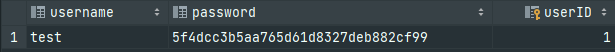
\includegraphics[width=1\linewidth]{no-salt.png} 
\centering
\caption{Bruges uden salt, oprettet i databasen}
\label{fig:no-salt}
\end{figure}

Ved at generere et MD5 hash med \verb|password| som input, og verificere at dette og hashet fra databasen er ens, kan man se at koden fungerer som ønsket. 

Derudover kan koden der opretter en bruger med salt også undersøges. Dette gøres igen ved at forsøge at oprette en bruger med navnet "test" og passwordet "password". Denne gang genererers et salt, som sættes bagefter passwordet inden det hashes. Databasen undersøge igen og resultatet kan ses på \figureautorefname{~\ref{fig:with-salt}}.

\begin{figure}[h]
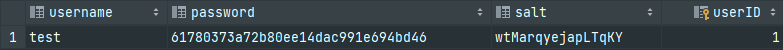
\includegraphics[width=1\linewidth]{with-salt.png} 
\centering
\caption{Bruges med salt, oprettet i databasen}
\label{fig:with-salt}
\end{figure}


Ved at generere et hash med passwordet og saltet uafhængigt af dette kode, er det igen tydeligt, at koden fungerer, da det genererede hash og hashet fra databasen er ens. 


\subsubsection{Hvorfor er det et problem?}
Det er et stort problem for sikkerheden, hvis der ikke bruges salt i en database \cite{noauthor_adding_nodate}. Hvis en ondsindet bruger fik adgang til at database med usaltede hashes, kunne en forespørgsel blot sendes til at database, der indeholder passwords og deres hash. Dette ville resulterer i, at man hurtigt kan finde en masse brugeres passwords. Hvis eksemplet fra testen bruges, kan man bruge en hjemmesiden som \verb|crackstation.net|, hvor man kan slå hashes op og få input teksten. Crackstation indeholder de mest brugte passwords og deres hashede værdier, man kan derfor slå et hash op og se hvad inputtet har været. Hvis man slår \verb|5f4dcc3b5aa765d61d8327deb882cf99| op, hvilket er hashet fra det usaltede password, viser den øjeblikkelig at input teksten var \verb|password|. 

Lidt af dette problem kan dog afdæmpes ved brug af salt, når man hasher passwordet. Hvis man slår \verb|61780373a72b80ee14dac991e694bd46| op på hjemmesiden, findes der ikke noget resultat - selvom det er det samme password. Salt er dog ikke hele løsningen på problemet, eftersom det er muligt at generere 21 milliarder hashes i sekundet, kan man blot 'genhashe' en masse password med saltet bagefter. Dette gør det dog meget langsommere at få passwords. Det betyder også, at en ondsindet bruger ikke kan få en masse brugere passwords ved blot at slå dem op på en hjemmeside, da der skal generes nye passwords for hver brugers salt. 


\subsubsection{Sammenligning med Django}
For at undersøge hvor virkelighedsnær koden i virkeligheden er, kan den eksempelvis sammenlignes med Django. Django er et webframework, der allerede har implementeret en sikker salt funktion. Et webframework er noget kode, der hjælper med at hoste en hjemmeside. Django er et populært webframework, som bliver brugt af en masse store virksomheder, heriblandt Instagram \cite{noauthor_django_nodate}. 

\begin{figure}[ht]
\begin{minted}[frame=lines,framesep=2mm,baselinestretch=1.2,linenos,breaklines]{python}
def md5(data=b"", *, usedforsecurity=True):
        return hashlib.md5(data)

def encode(self, password, salt):
    self._check_encode_args(password, salt)
    hash = md5((salt + password).encode()).hexdigest()
    return "%s$%s$%s" % (self.algorithm, salt, hash)
\end{minted}
\caption{Djangos implementation af MD5 hashing \cite{noauthor_django_2022-2}\cite{noauthor_django_2022}}
\label{code:django-md5}
\end{figure}

Koden vist i \figureautorefname{~\ref{code:django-md5}} er hentet fra Djangos officielle GitHub side. Koden er spredt ud over to forskellige filer, og filerne indeholder meget andet kode, hvilket er derfor der bliver kaldt nogle funktioner, som ikke er beskrevet her. De viste to funktioner er dog de vigtigste i forhold til MD5, hvilket er derfor de er blevet valgt. 

\begin{figure}[ht]
\begin{minted}[frame=lines,framesep=2mm,baselinestretch=1.2,linenos,breaklines]{python}
letters = string.ascii_letters  
salt = "".join(random.choice(letters) for i in range(16))  

hashed_password = hashlib.md5((password + salt).encode()).hexdigest()
\end{minted}
\caption{Kode skrevet til virkelighednær implementation af MD5, samme kode vist i \figureautorefname{~\ref{code:create-user-w-salt}}}
\label{code:django-comp-code}
\end{figure}

Begge implementationer minder meget om hinanden, da de begge bruger \verb|hashlib| biblioteket, til at hashe teksten. I Django implementationen oprettes der en funktion, som hedder \verb|md5()|, de blot kalder hashlib funktionen, som faktisk beregner MD5 hashet. 

Derudover oprettes der en funktion, som hasher passwordet med et salt, og retunerer det i et specifik format. Denne funktion kan ses på \figureautorefname{~\ref{code:django-md5}} linje 4 - 7. Koden på linje 5, er blot en intern metode i klassen, der tjekker om passwordet og saltet lever op til deres krav. På linje 6 hashes passwordet sammen med saltet. Det sker på samme måde som i \figureautorefname{~\ref{code:django-comp-code}}, blot hvor saltet og passwordets plad har byttet plads. 

Django implementationen bruger en general salting funktion, der kan bruges til alle deres algoritmer. Derudover er det en hashing funktion, der er mere sikker, fordi den er designet med sikkerhed i mende. Salt funktionen i \figureautorefname{~\ref{code:django-comp-code}} er meget usikker i forhold til Djangos funktion. Salt funktionen i \figureautorefname{~\ref{code:django-comp-code}} er usikker fordi den udnytter \verb|random| bibliotektet, som er frarådet at bruge til sikkerheds applikationer \cite{noauthor_random_nodate}.

I linje 7 på \figureautorefname{~\ref{code:django-md5}} retuneres algoritmen, hashet og saltet adskildt med \$. Dette bruger de i deres andre funktioner og er derfor ikke releveant i forhold til koden udviklet til SOP'en. 

\subsection{Kollisioner}
Som beskrevet i afsnittet om hashing algoritmer er en hash kollision en situation hvor to forskellige input giver det samme output (samme hash). I den virkelig verden burde dette være statistik usandsynligt tilfældigvis at støde på en hash kollision, da der er $2^{128}$ mulige hashes, men forskere har fundet sårbarheder i MD5 algoritmen, der gør det muligt at fremskynde sådan en hash kollision. Dette undersøges dybdegående i afsnit 8, om MD5 kollisioner. 


\section{Brug af MD5}
\subsection{Brug i fortiden}
MD'et i MD5 står for "message digest". MD5 er den femte udvikling af MD algoritmerne. De er udviklet af Ron Rivest, som også har udviklet andre vigtige algoritmer inden for computersikkerhed. De første fire versioner af MD algoritmerne blev aldrig rigtig brugt. De første tre algoritmer, var så usikre at de knap nok nåede ud af udviklingsprocessen før en kollision blev opdaget. MD4 holdt cirka et år. MD5 var en sikker hashing algoritme indtil de første år af 2000. \cite{lake_what_2021}

Indtil sommeren 2013, brugte Yahoo MD5 til at hashe deres brugeres passwords \cite{noauthor_yahoo_nodate}.

\subsection{Brug i nutiden}
I dag er de helt store platforme gået væk fra brugen af MD5 i deres systemer. Der findes dog stadig mange hjemmesider og systemer der bruger MD5 som en sikkerhedsforanstaltning, eksempelvis CMS'er CMS står for Content Management System og er noget software der kan hjælpe med at organisere indhold på hjemmesider. De fleste af disse CMS'er kan også bruges til at opbygge hele hjemmesider. 

En undersøgelse fra Universitetet i Piraeus viser, at mange store CMS'er stadig bruger MD5 som deres standard hashing algoritme. Mange bruger dog et 'salt' som øger sikkerheden en lille smule \cite{ntantogian_evaluation_2019}.

En af de helt store CMS'er i verden, Wordpress, bruger stadig MD5 som deres standard hashing algoritme. Det er estimeret, at cirka 31\% af hele internettet bruger Wordpress som base. Det betyder også, at cirka 31\% af verdens hjemmesider bruger en gammel usikker hashing algoritme. Det er dog langt fra alle hjemmesider der er udsat, da mange folk bruger Wordpress til deres simple hjemmesider, hvor ingen skal logge ind. Dog er der stadig en massiv mængde af internettet der bruger en usikker algoritme. \cite{ntantogian_evaluation_2019}

Wordpress bruger dog et salt til at gøre det mere sikkert. Derudover kører de hashing algoritmen 8192 gange på passwordet. De tager altså outputet af den første algoritme og bruger det som input - det gør de 8192 gange. Dette kaldes for en \verb|iteration|. Det er en sikkerhedsforanstaltning, der gør det sværere at 'gætte' passwordet, da algoritmen skal køres 8192 gange. På den anden side er minimum password længden kun en enkelt karakter, hvilket betyder, at mange folk sandsynligvis vælger et kort og usikkert password. Det betyder at der er langt færrer sandsynlige passwords, der skal hashes, for at finde det tilhørende password.

Rapporten fra universitetet estimerer, at hvis man opnår adgang til en Wordpress database, kan 41,5\% af passwords i gennemsnit gættes inden for 2,4 sekunder, fordi de har så usikkert et system \cite{ntantogian_evaluation_2019}.

\subsection{Brug i fremtiden}
I fremtiden gøres der sandsynligvis ikke brug af MD5 i nogle sikkerhedsmæssige sammenhænge. Udviklere og programmørere ved efterhånden godt, at MD5 er usikker og ikke burde bruges. Det er også sandsynligvis grunden til, at MD5, hovedsagligt bliver brugt i gamle applikationer, hvor det kræver for meget arbejde (eller er helt umuligt) at skifte fra MD5. Hvis en platform allerede bruger MD5, og alle platformens brugers passwords er hashet med MD5, kan det være et utrolig stort arbejde at skifte til en helt anden hashing algoritme. 

Det er dog ikke umuligt at skifte hashing algoritme. En af de mest udsatte CMS'er på listen, "Composr", brugte tidligere en enkelt iteration af MD5, men har efterfølgende skiftet til en anden og mere sikker hashing algoritme. De bruger stadig MD5 til de ældre brugere, der endnu ikke er skiftet. Derudover bruger de MD5 som en fallback, hvis deres nye algoritme skulle fejle. I deres nyere versioner er det heller ikke muligt at vælge MD5 som hashing algoritme. \cite{noauthor_composr_nodate}

Som computere bliver bedre og kraftigere, bliver de algoritmer vi synes er sikre i dag, sikkert også usikre. Engang var MD5 helt fint at bruge i sikkerhedsapplikationer, men eftersom computere blev hurtigere og forskere brugte tid på at undersøge algoritmen, blev det usikkert at bruge MD5. Det samme kommer sikkert til at ske for alle de "sikre" algoritmer i dag, det er derfor vigtigt, at man husker at følge med tiden.

\section{MD5 kollisioner}
\subsection{Intro}
Som tidligere beskrevet i intro om usikkerheder i MD5 er en kollision, hvor to forskellige input, giver samme MD5 hash. Ofte bruges to forskellige filer som input, det er derfor muligt at have to forskellige billeder med ens hash.  

\subsection{Teori}
Selvom MD5 er erklæret usikkert af mange cybersikkerhedsforskere, er det stadig storset umuligt at vælge et hash til en fil. Det er muligt at lave kollisioner mellem to filer, men det er stadig ikke muligt at vælge et specifikt hash. \cite{noauthor_hash_2022}

\footnotetext[8]{Denne struktur er naturligvis stadig kompliceret, men kollisionen mellem PNG'er er nemmere at fremvise og forestå i forhold til mere komplicerede formater, som MP4 eller ZIP filer}

\footnotetext[9]{En blok er en del af formatet, der specificere noget specielt om filen. I PNG formatet er der eksempelvis en blok, som definerer højden og bredden af billedet.}

Til dette forsøg på at generere en MD5 kollision, anvendes to billeder med PNG formatet. Dette gøres, da det er en filtype, der har let forståelig stuktur\footnotemark[8]. Derudover er det nemmere at vise at der ingen forskel er på indholdet af filen, ved at se på billederne. 

En hash kollision fungerer ved at indsætte noget specielt tekst (for mennesker ligner det noget helt tilfældig tekst) i en kommentar sektion af filerne. Disse kommentar sektioner er ikke en officiel del af filtype specifikationen, men mange programmer, der skal forestå og tolke filen, læser forbi "kommentar sektionen". I PNG formatet ignoreres alle "blokke"\footnotemark[9] der ikke starter med et stort bogstav. \cite{noauthor_hash_2022}

Med en kollision af filerne sættes filerne i forlængelse af hinanden, da det er nemmere at lave identiske hashes, når indholdet er mere ens. Der bruges så en kommentar sektion til at udkommenterer den del af, filen der ikke skal vises. Hvis men eksempelvis har to billeder, sættes de i forlængelse af hinanden. Billedefremvisernen viser kun det første billede, der ses i filen. Ved at bruge kommentar sektionen kan man ugyldiggøre det første billede, så billedefremviseren læser forbi det og kun viser det andet billede. \cite{noauthor_hash_2022}

Der findes forskellige strategier til at kollidere to filer, således at de får samme hash. Til dette forsøg bruges en strategi, der hedder "UniColl", som er en af de hurtigtste måder at kollidere to filer. UniColl er ikke godt, hvis man skal have fleksibilitet, som eksempelvis at kollidere to forskellige filtyper. Eftersom der blot skal kollideres to billeder, er UniColl brugbart.  


\subsection{Forsøg på MD5 kollision}
Til at kollidere de to billeder bruges kode der er skrevet i Python \cite{noauthor_hash_2022-1}.
For at dette kode kan fungere, skal der bruges et eksternt program til at lave selve kollisionen. Kollisionen samles til en fil, med det rigtige hash. I dette forsøg fokuseres der på koden, som samler resultatet fra UniColl til en fil med det rigtige hash. 

\subsubsection{Kollisionen}
Først findes to billeder der skal kollideres. Til dette forsøg er det to simple billeder som kan ses på \figureautorefname{~\ref{fig:coll-before}}, der tydeligvis er forskellige. Det betyder også, at de har forskellige hashes henholdsvis \verb|1b77763185a434d10ab20fde9468c514| og \verb|b380ad35e135f23a1fe2211ed0306d77|. 

\begin{figure}[!h]
    \centering
    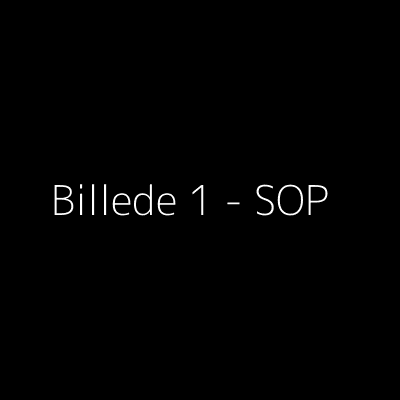
\includegraphics[width=5cm]{no.png}
    \qquad
    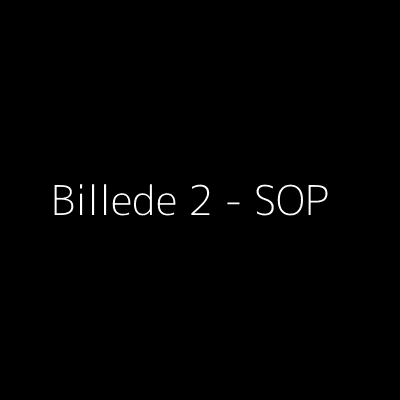
\includegraphics[width=5cm]{yes.png}
    \caption{Billeder til kollision, før kollision}
    \label{fig:coll-before}
\end{figure}

Ved at køre Python koden køres også UniColl, som laver en kollision, hvorefter python koden, samler resultatet til de samme billeder som før blot med ens hash. Det kan gøres ved at køre kommandoen: \verb|python3 stdPng.py img1.png img2.png|. Koden tager to argumenter (to input), som er de to billeder, der skal kollideres. Efter at have kørt koden og ventet på at UniColl færdiggører sin process, resulterer det i to billeder. Disse billeder kan ses på \figureautorefname{~\ref{fig:coll-after}}.

\begin{figure}[!h]
    \centering
    \includegraphics[width=5cm]{0c3a2938-1.png}
    \qquad
    \includegraphics[width=5cm]{0c3a2938-2.png}
    \caption{Billeder til kollision, efter kollision}
    \label{fig:coll-after}
\end{figure}

Billederne på \figureautorefname{~\ref{fig:coll-after}} ser identiske ud som dem i \figureautorefname{~\ref{fig:coll-before}}. 

De har dog begge hashet \verb|c8b4c751c71b42fcf96390eef7bc86ee|.
Det betyder derfor at kollisionen er lykkedes. Eftersom begge billeder indeholder hinanden, er det fordoblet i størrelse. En kollision kan være et sikkerhedsproblem, da det kan betyde, at to forskellige filer (eksempelvis en virus og et normalt program) kan have samme hash.


\subsubsection{Kode}
For at kunne bruge koden ordenligt, er det vigtigt at forestå den. På \figureautorefname{~\ref{code:coll-code}} ses et uddrag af Python koden det lavede kollisionen. 

\begin{figure}[ht]
\begin{minted}[frame=lines,framesep=2mm,baselinestretch=1.2,linenos,breaklines]{python}
def get_data(args):
  fn1, fn2 = args

  with open(fn1, "rb") as f:
    d1 = f.read()
  with open(fn2, "rb") as f:
    d2 = f.read()

  assert d1.startswith(b"\x89PNG\r\n\x1a\n\x00\x00\x00\rIHDR")
  assert d2.startswith(b"\x89PNG\r\n\x1a\n\x00\x00\x00\rIHDR")

  assert d1[:0x21] == d2[:0x21]

  return d1, d2
\end{minted}
\caption{Uddrag fra kollisions koden \cite{noauthor_hash_2022-1}}
\label{code:coll-code}
\end{figure}

Koden vist i \figureautorefname{~\ref{code:coll-code}} er funktionen, der henter billederne, man sender med, når man kører koden. Da \verb|args| bliver sendt som et array med to elementer, kan de to elementer gives en variabel hver. Dette gøres i linje 2. 

I linje 4 og 5 åbnes filen, der er specificeret i \verb|fn1|. Den åbnes i \verb|rb| mode, hvilket betyder "read bytes", så man læser de rå bytes. Filen bliver gemt i variablen \verb|f|. I linje 5 bliver indholdet af filen læst over i variablen \verb|d1|. 
Det samme sker for den anden fil i linjerne 6-7.

I linje 9 - 10 tjekkes der om begge filer starter med standard PNG header, der specificerer at det er en PNG fil. \verb|assert| keywordet tjekker om det kode der stå bagefter er sandt, og stopper eksekveringen af programmet, hvis det er falsk. I denne situation vil programmet stoppe, hvis begge filer ikke indeholder PNG headeren. 

I linje 12 tjekkes om begge filer indeholder samme start. Det kan gøres i Python ved at indekse fra 0 til 0x21 med følgende syntax \verb|[:0x21]|. 

Til sidst returnerer funktionen indholdet af de to filer. 

\section{Konklusion}
I denne rapport er der blevet redegjort, diskuteret og analyseret MD5 algoritmen. Efter undersøgelsen er det tydeligt, at MD5 er en fundamental usikker algoritme, om hverken burde bruges til checksum eller hashing af passwords (eller anden sensitiv data), da der er flere sårbarheder i algoritmen. Disse sårbarheder indebærer hurtig generering af MD5 hashes, hvilket er et problem, hvis en ondsindet bruger får adgang til en database indeholdende eksempelvis brugernavne og passwords. Det er derfor muligt at hashe mange kendte passwords, hvoraf nogle af dem sandsynligvis vil kunne findes i databasen. For at gøre databaserne mere sikre, blev der opfundet et "salt", som er en tilfældig streng af tekst, der sættes foran eller bagved passwordet, inden det hashes. Dette gør passwords hashes mere sikre, men eftersom det er muligt at generere mange hashes indenfor kort tid, hjælper denne løsning ikke helt. 

Derudover er der blevet demonstreret en anden sårbarhed, som er MD5 kollisioner. En MD5 kollision er beskrevet som to forskellige input i hashing funktionen, der resulterer i samme output. I denne rapport er der blevet lavet en kollision mellem to forskellige billeder. En kollision er ikke en ligeså stor sårbarhed, som hurtig generering af hashes, men er stadig et stort problem. Dette er et stort problem, da man ikke med sikkerhed kan fastslå om en given fil har det forventede indhold. Det er eksempelvis muligt at lave en hash kollision mellem et sikkert program og en virus. 


\bibliographystyle{dk-apali}
\bibliography{sop}

\newpage
\appendix
\section{Kode}
\subsection{Virkelighedsnær Implementation af MD5 i Python}
\begin{minted}[mathescape,autogobble,escapeinside=``,frame=lines,framesep=2mm,baselinestretch=1.2,linenos,breaklines]{python}
import hashlib
import sqlite3
import string
import random

try:  # Prøver at oprette forbindelse til databasen og laver to tabeller
    # Forbinder til databasen og laver den hvis den ikke findes
    conn = sqlite3.connect('database.db')
    # Laver en cursor, som er en måde at hente og skrive til databasen
    c = conn.cursor()
    print("Created and connected to database")

    # Laver en tabel med brugernavn, password og salt hvis den ikke findes. Skrevet i SQL.
    t = 'CREATE TABLE IF NOT EXISTS saltedCredentials (username VARCHAR (32), password VARCHAR (32), salt VARCHAR (32), userID INTEGER PRIMARY KEY AUTOINCREMENT) '

    # Kører SQL kommandoen beskreven i t
    c.execute(t)

    # Opdaterer databasen med den nye SQL kommando
    conn.commit()
    print("Created table with salted credentials")

    # laver en tabel med brugernavn og password hvis den ikke findes
    t = 'CREATE TABLE IF NOT EXISTS credentials (username VARCHAR (32), password VARCHAR (32), userID INTEGER PRIMARY KEY AUTOINCREMENT)'

    # Kører SQL kommandoen beskreven i t
    c.execute(t)

    # Opdaterer databasen med den nye SQL kommando
    conn.commit()
    print("Created table with credentials")

except Exception as e:  # Hvis der er en fejl, så printes den
    print(e)


def create_user_salted(username, password):
    # Genererer et tilfældigt salt
    letters = string.ascii_letters  # Laver en string med alle bogstaver i alfabetet
    salt = "".join(random.choice(letters) for i in range(16))  # Laver en string med 16 tilfældige bogstaver fra "letters"

    # Lægger saltet til passwordet og laver det om til bytes så det kan hashes
    hashed_password = hashlib.md5((password + salt).encode()).hexdigest()

    # Laver en SQL kommando der henter alle brugernavnet brugeren har indsat
    c.execute("SELECT * FROM saltedCredentials WHERE username = ?", (username,))
    if c.fetchone() is None:  # Hvis der ikke er nogen brugere med det brugernavn
        # Laver en SQL kommando der indsætter brugernavn, password og salt i databasen
        c.execute("INSERT INTO saltedCredentials(username,password,salt) VALUES (?,?,?)", (username, hashed_password, salt))
        conn.commit()
        print(f"User {username} created, with salt")
    else:  # Printer at der allerede er en bruger med det brugernavn, hvis der er
        print("User already exists")


def create_user(username, password):
    # Hasher passwordet
    hashed_password = hashlib.md5(password.encode()).hexdigest()

    # Laver en SQL kommando der henter alle brugernavnet brugeren har indsat
    c.execute("SELECT * FROM credentials WHERE username = ?", (username,))
    if c.fetchone() is None:  # Hvis der ikke er nogen brugere med det brugernavn
        # Laver en SQL kommando der indsætter brugernavn og password i databasen
        c.execute("INSERT INTO credentials(username,password) VALUES (?,?)", (username, hashed_password))
        conn.commit()
        print(f"User {username} created")

    else:  # Printer at der allerede er en bruger med det brugernavn, hvis der er
        print("User already exists")


def authenticate_user(username, password):
    try:  # Prøver at hente passwordet fra databasen med en SQL kommando
        c.execute("SELECT password FROM credentials WHERE username = ?", (username,))
        fetched_password = c.fetchone()[0]  # siden der kun er et resultat, så hentes det første element i tuplen

    except TypeError:  # Skriver at brugeren ikke findes hvis der ikke er nogen brugere med det brugernavn
        print("Could not fetch password - user does not exist")
        return  # Stopper funktionen

    # Initialiserer en variable med det hashede password.
    # Passwordet fra brugeren, bliver lavet om til bytes via .encode() metoden
    hashed_password = hashlib.md5(password.encode()).hexdigest()

    # Tjekker om passwordet er det samme som det gemte og printer resultatet
    if hashed_password == fetched_password:
        print("User authenticated")
    else:
        print("User not authenticated")

    input("Press enter to exit")  # Stopper eksekveringen af programmet indtil brugeren trykker på en tast


def authenticate_user_salted(username, password):
    try:  # Prøver at hente passwordet og saltet fra databasen med en SQL kommando
        c.execute("SELECT salt FROM saltedCredentials WHERE username = ?", (username,))
        salt = c.fetchone()[0]  # siden der kun er et resultat, så hentes det første element i tuplen

        # Henter det hashede password fra databasen
        c.execute("SELECT password FROM saltedCredentials WHERE username = ?", (username,))
        fetched_password = c.fetchone()[0]

    except TypeError:  # Skriver at brugeren ikke findes hvis der ikke er nogen brugere med det brugernavn
        print("Could not fetch salt or password - user does not exist")
        return  # Stopper funktionen

    # Initialiserer en variable med det hashede password.
    # Passwordet fra brugeren sammen med hashed fra databasen, bliver lavet om til bytes via .encode() metoden
    hashed_password = hashlib.md5((password + salt).encode()).hexdigest()

    # Tjekker om passwordet er det samme som det gemte og printer resultatet
    if hashed_password == fetched_password:
        print("User authenticated")

    else:
        print("User not authenticated")

    input("Press enter to exit")  # Stopper eksekveringen af programmet indtil brugeren trykker på en tast


def fetch_user_creds():  # Funktion der henter brugernavn og password fra brugeren
    username = input("Username: ")
    password = input("Password: ")

    return username, password


def main():
    print("""
    Welcome!
    Press the corresponding number to do the following:
        1. Create a user
        2. Create a user with salt
        3. Authenticate a user
        4. Authenticate a user with salt
    
    n. Exit
    """)
    choice = input("Number: ")

    if choice == "1":
        username, password = fetch_user_creds()  # Henter brugernavn og password fra brugeren
        create_user(username, password)
    elif choice == "2":
        username, password = fetch_user_creds()

        create_user_salted(username, password)

    elif choice == "3":
        username, password = fetch_user_creds()
        authenticate_user(username, password)

    elif choice == "4":
        username, password = fetch_user_creds()
        authenticate_user_salted(username, password)

    else:
        exit()


if __name__ == "__main__":
    while True:
        main()


    
\end{minted}


\end{document}